\documentclass{beamer}
\usepackage[latin1]{inputenc}
%\usetheme[noshadow,nonav,nologo]{NYU}
\usenavigationsymbolstemplate{}
\usetheme[numbers]{NYU}
\usepackage{amsmath}
\usepackage{amsfonts}
\usepackage{amssymb}
\usepackage{color, colortbl}
\usepackage{graphicx}
\usepackage{subfigure}
\usepackage{caption}
\usepackage{multirow}
\usepackage{lmodern}
\usepackage{subcaption}
\usepackage{epstopdf}
\DeclareMathOperator*{\argmax}{arg\,max}


\makeatletter
\newcommand{\thickhline}{%
    \noalign {\ifnum 0=`}\fi \hrule height 2pt
    \futurelet \reserved@a \@xhline}

\title{Unsupervised Learning of Deep Feature Hierarchies from Unlabeled Video Data}
\date{ Courant Institute of Mathematical Sciences \\ \vspace{0.2cm} September 2015} 
\author{Ross Goroshin}

\begin{document}
\begin{frame}
\titlepage
\end{frame}

\begin{frame}
\begin{center} 
\huge \color{blue} \emph{Research Background}
\end{center} 
\end{frame} 

\begin{frame}
\begin{columns}[T] % align columns
\begin{column}{.33\textwidth}
\color{blue}\rule{\linewidth}{2pt}
\tiny{Visibility Path Planning via Variational Optimization }
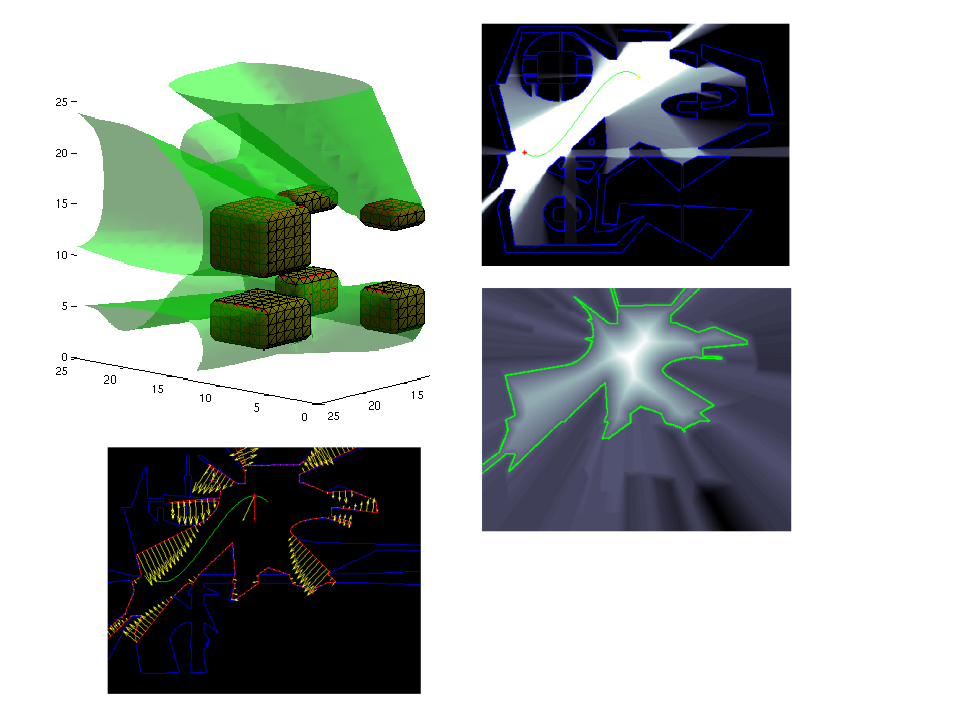
\includegraphics[scale=0.3,trim = 1 30 1 1, clip]{./Figures/vis.pdf}
\end{column}%
\hfill%
\begin{column}{.33\textwidth}
\color{blue}\rule{\linewidth}{2pt}
\tiny{Cable Detection in Sonar Imagery}
\centering
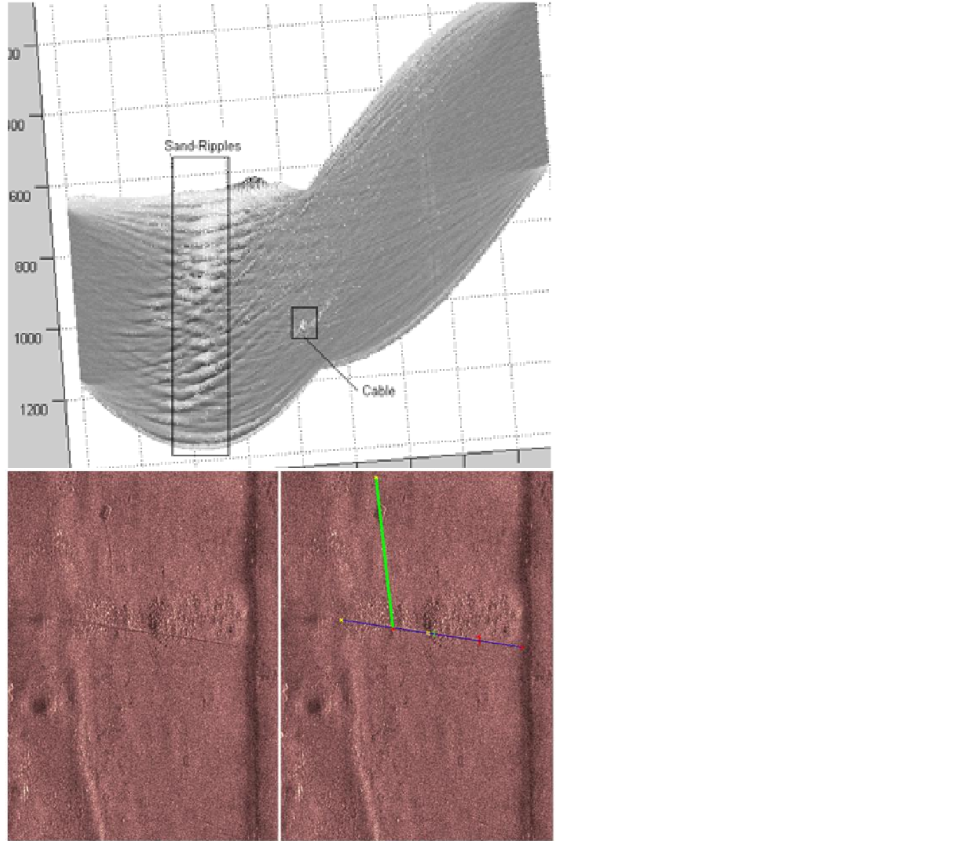
\includegraphics[scale=0.30,trim = 1 1 200 40, clip]{./Figures/cable.pdf}
\end{column}%
\begin{column}{.33\textwidth}
\color{blue}\rule{\linewidth}{2pt}
\tiny{Segmentation with Active-Contours}
\centering
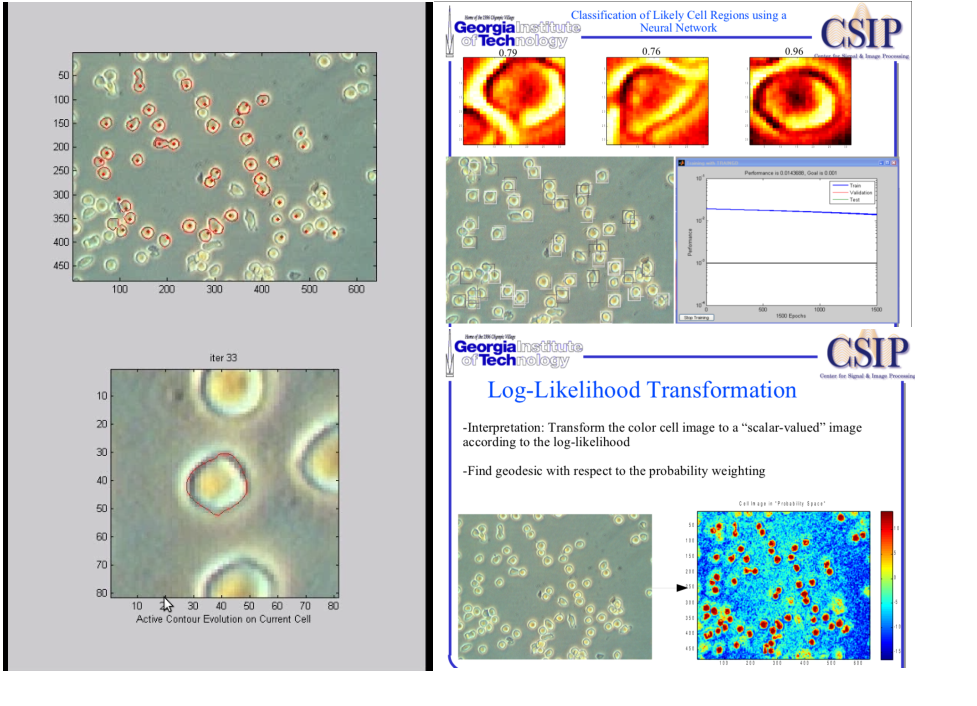
\includegraphics[scale=0.35,trim = 1 1 260 10, clip]{./Figures/cells.pdf}
\end{column}%
\end{columns}
\vspace{0.5cm} 
\begin{columns}[T] % align columns
\begin{column}{.48\textwidth}
\color{blue}\rule{\linewidth}{2pt}
\tiny{Monocular Obstacle Detection}
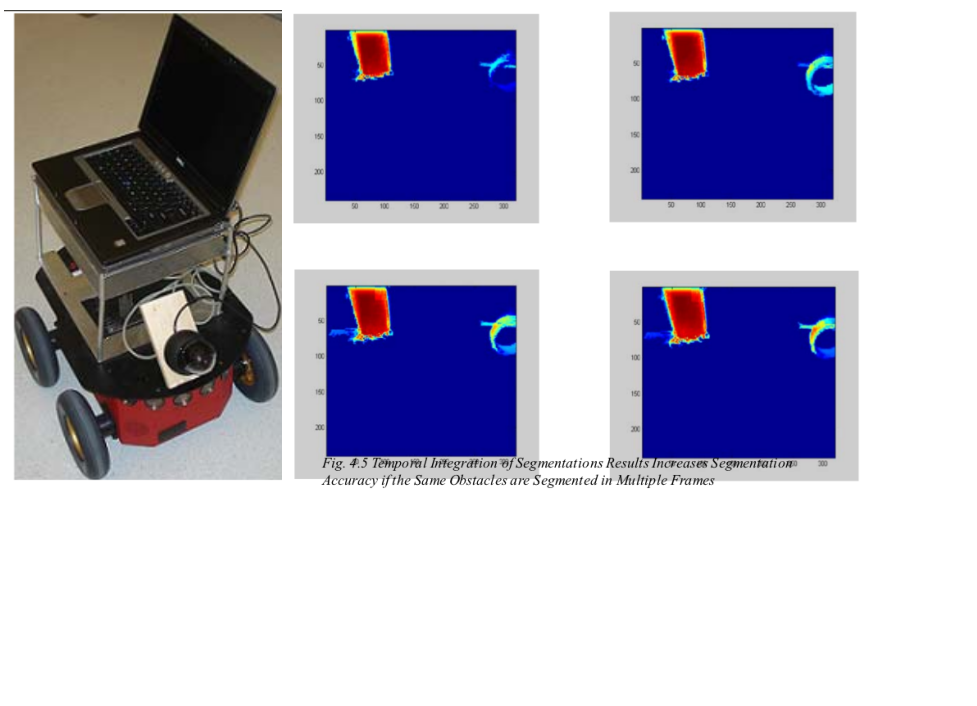
\includegraphics[scale=0.40,trim = 1 1 30 10, clip]{./Figures/obs.pdf}
\end{column}%
\hfill%
\begin{column}{.48\textwidth}
\color{blue}\rule{\linewidth}{2pt}
\tiny{Synthetic Aperture Sonar Imaging}
\centering
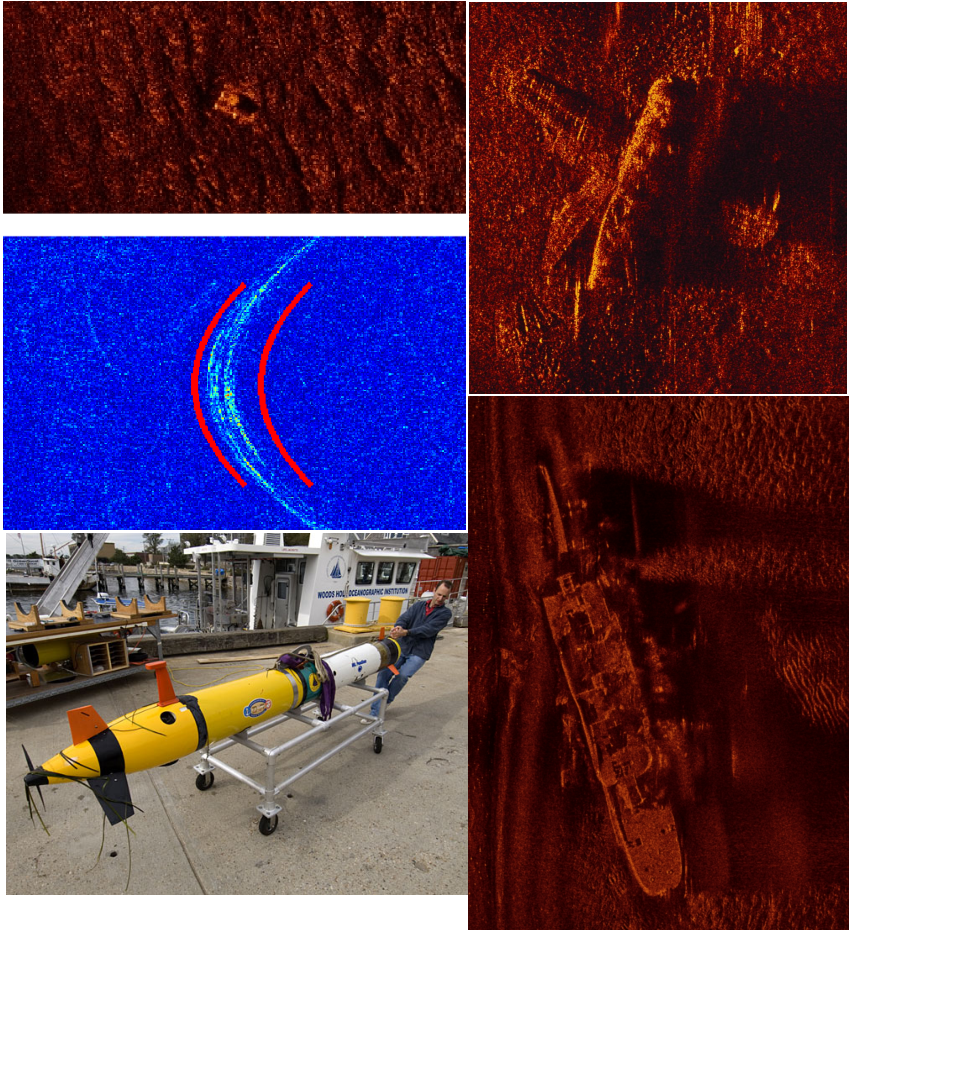
\includegraphics[scale=0.22,trim = 1 1 60 10, clip]{./projects_slide/sas.pdf}
\end{column}%
\end{columns}
\end{frame}

\begin{frame}
\begin{center} 
\huge \color{blue} \emph{Deep Learning for Computer Vision}
\end{center} 
\end{frame} 

\begin{frame}
\frametitle{Classic Computer Vision Pipeline}
\begin{center} 
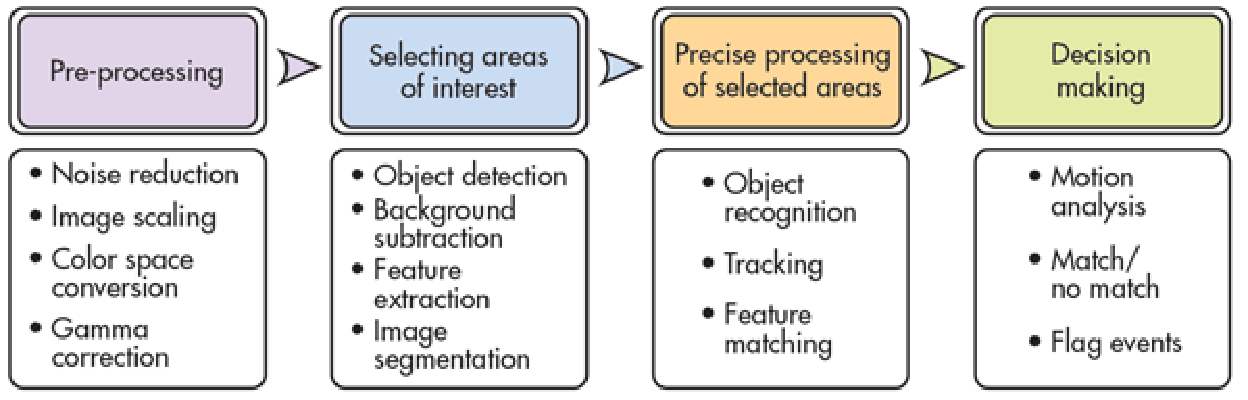
\includegraphics[scale=0.31]{./Figures/old_pipeline.pdf} \\ \vspace{0.5cm} 
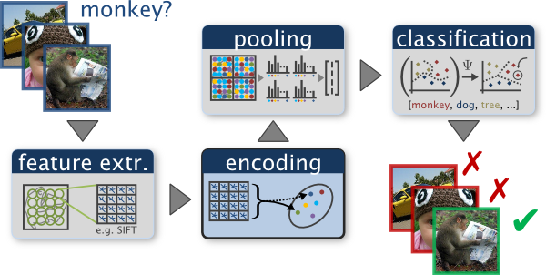
\includegraphics[scale=0.6]{./Figures/detection.pdf} \hspace{1.5cm} 
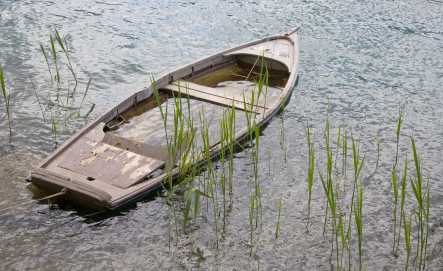
\includegraphics[scale=0.5]{./Figures/boat.jpg}\\
The engineer must manually plug all the ``leaks'' in the pipeline \\ \vspace{0.5cm} 
\tiny{http://cs.brown.edu/courses/cs143/}
\end{center} 
\end{frame} 

\begin{frame}
\frametitle{Computer Vision as of 2012}
\begin{columns}[T] % align columns
\begin{column}{.4\textwidth}
\begin{itemize} 
\item{Leverage machine learning to plug the leaks with data}
\item From engineering features $\rightarrow$ engineering \emph{feature learning architectures}   
\end{itemize} 
\centering
\color{blue}\rule{\linewidth}{2pt} \tiny{Krizhevsky, \emph{NIPS 2012}} 
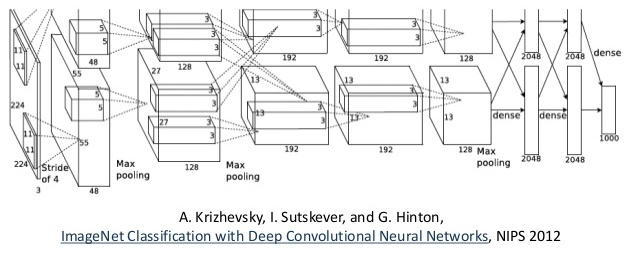
\includegraphics[scale=0.25]{./Figures/alexNet.jpg}
\end{column}%
\hfill%
\begin{column}{.6\textwidth}
\color{blue}\rule{\linewidth}{2pt}
\tiny{Tompson, Goroshin, Jain, LeCun, Bregler. \emph{CVPR 2015}}
\centering
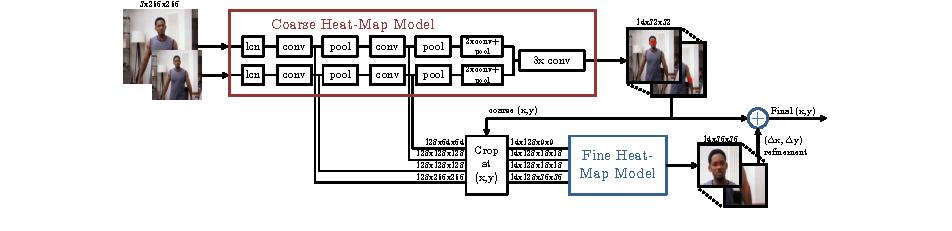
\includegraphics[scale=0.4]{./Figures/network2.pdf} \\
\tiny{Socher, Huval, Bhat, Manning, Ng. \emph{NIPS 2012}}   
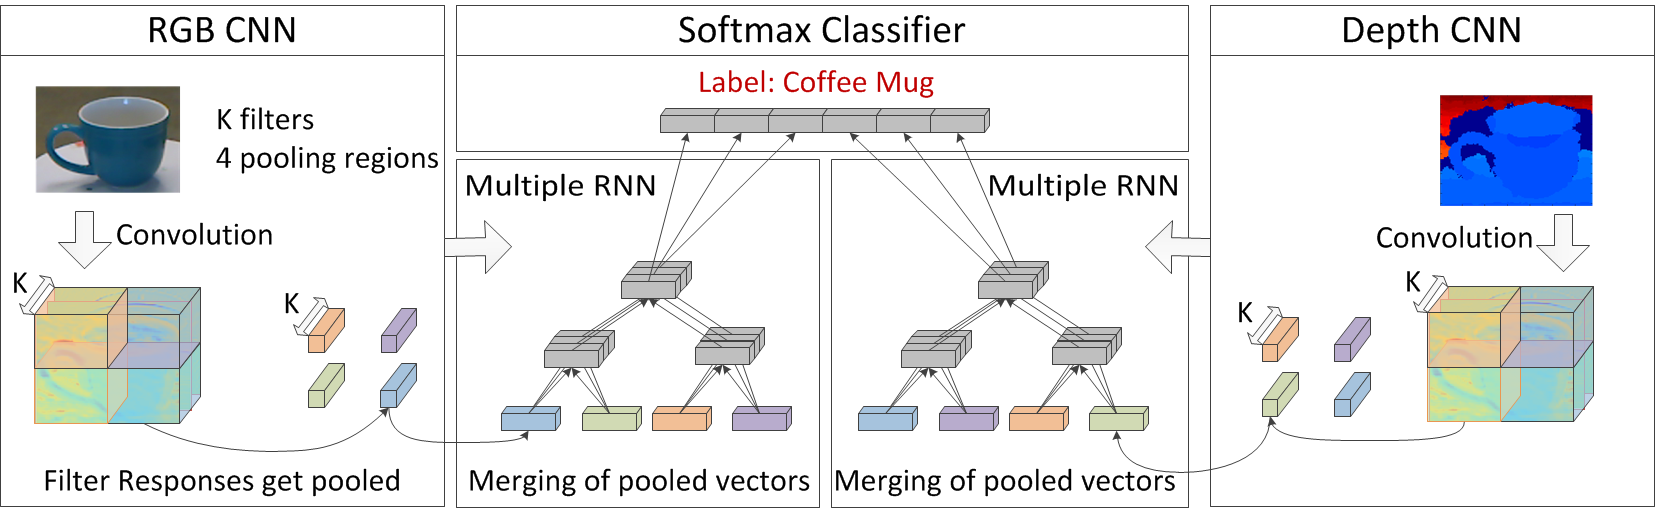
\includegraphics[scale=0.15]{./Figures/socher.png} \\
\tiny{Eigen, Puhrsch, Fergus. \emph{NIPS 2014}} \\
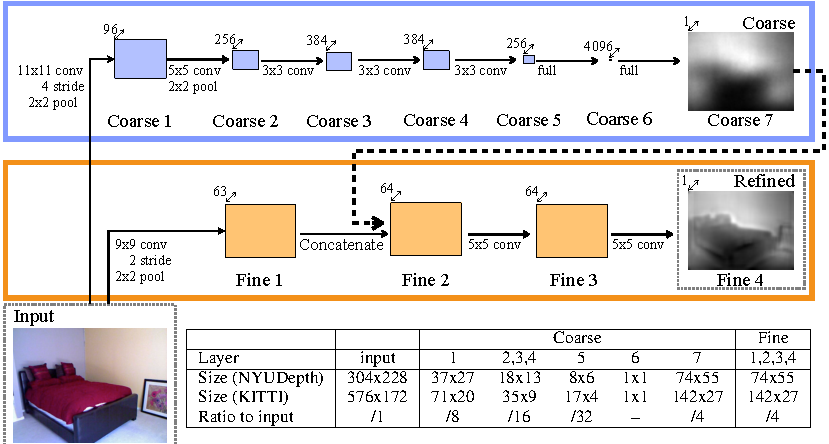
\includegraphics[scale=0.35]{./Figures/network3.pdf} \\
...and many more 
\end{column}
\end{columns}
\end{frame} 

\begin{frame}
\frametitle{Example: Human Pose Estimation}
\tiny{ \color{blue} \textbf{Tompson, Goroshin, Jain, LeCun, Bregler. \emph{CVPR 2015}}}
\begin{center} 
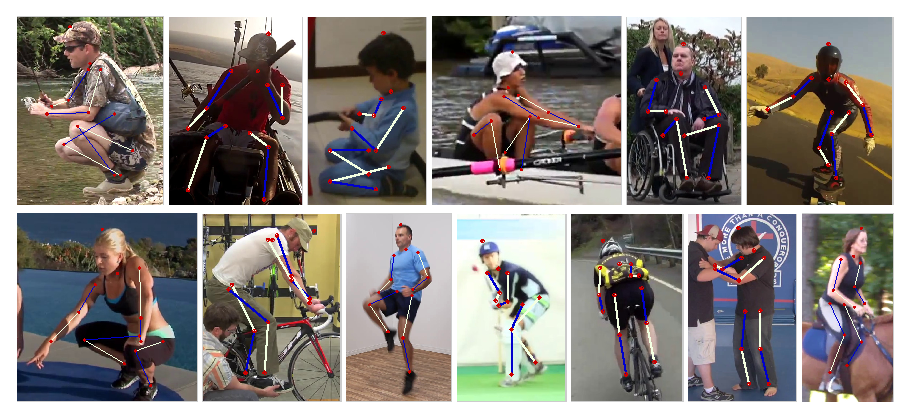
\includegraphics[scale=0.40]{./Figures/joints.pdf}
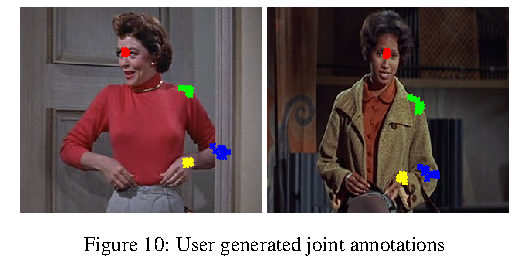
\includegraphics[scale=0.40]{./Figures/human.pdf}\\
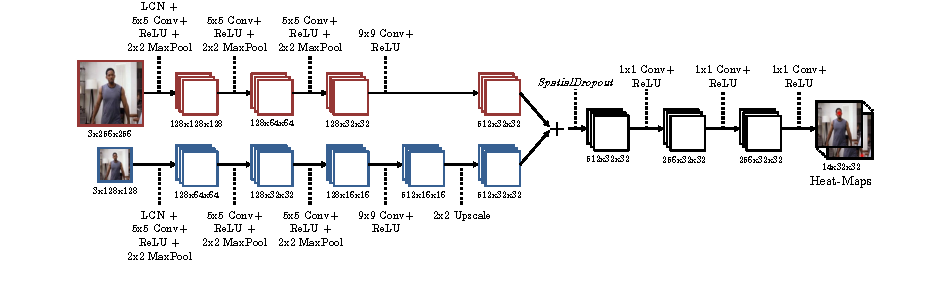
\includegraphics[scale=0.50]{./Figures/network.pdf}\\
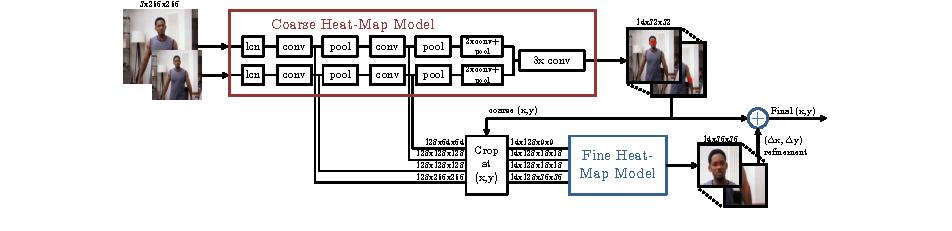
\includegraphics[scale=0.70]{./Figures/network2.pdf}\\
\end{center} 
\end{frame} 

\begin{frame}
\begin{center} 
\huge \color{blue} \emph{Unsupervised Feature Learning}
\end{center} 
\end{frame} 

\begin{frame}
\frametitle{Generically useful Feature Representations} 
\begin{itemize} 
\item{Experiments show that feature hierarchies are transferable}
\item{Natural learning machines don't need $10^6$ labeled examples}
\item{Is there an objective that allows us to learn high-level task-agnostic representations?}
\item{Leverage virtually infinite amount of unlabeled data \bf $\rightarrow$ reduce training time, obtain better generalization, and enable on-line learning/adaptation}
\end{itemize} 
\centering
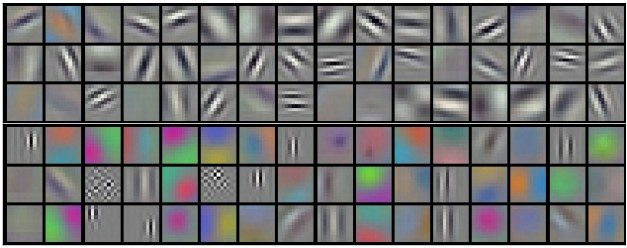
\includegraphics[scale=0.25]{./Figures/weights.jpeg} \\
\emph{\tiny{Krizhevsky et al. NIPS 2012}} 
\end{frame} 

\begin{frame} 
\frametitle{Representation Learning}
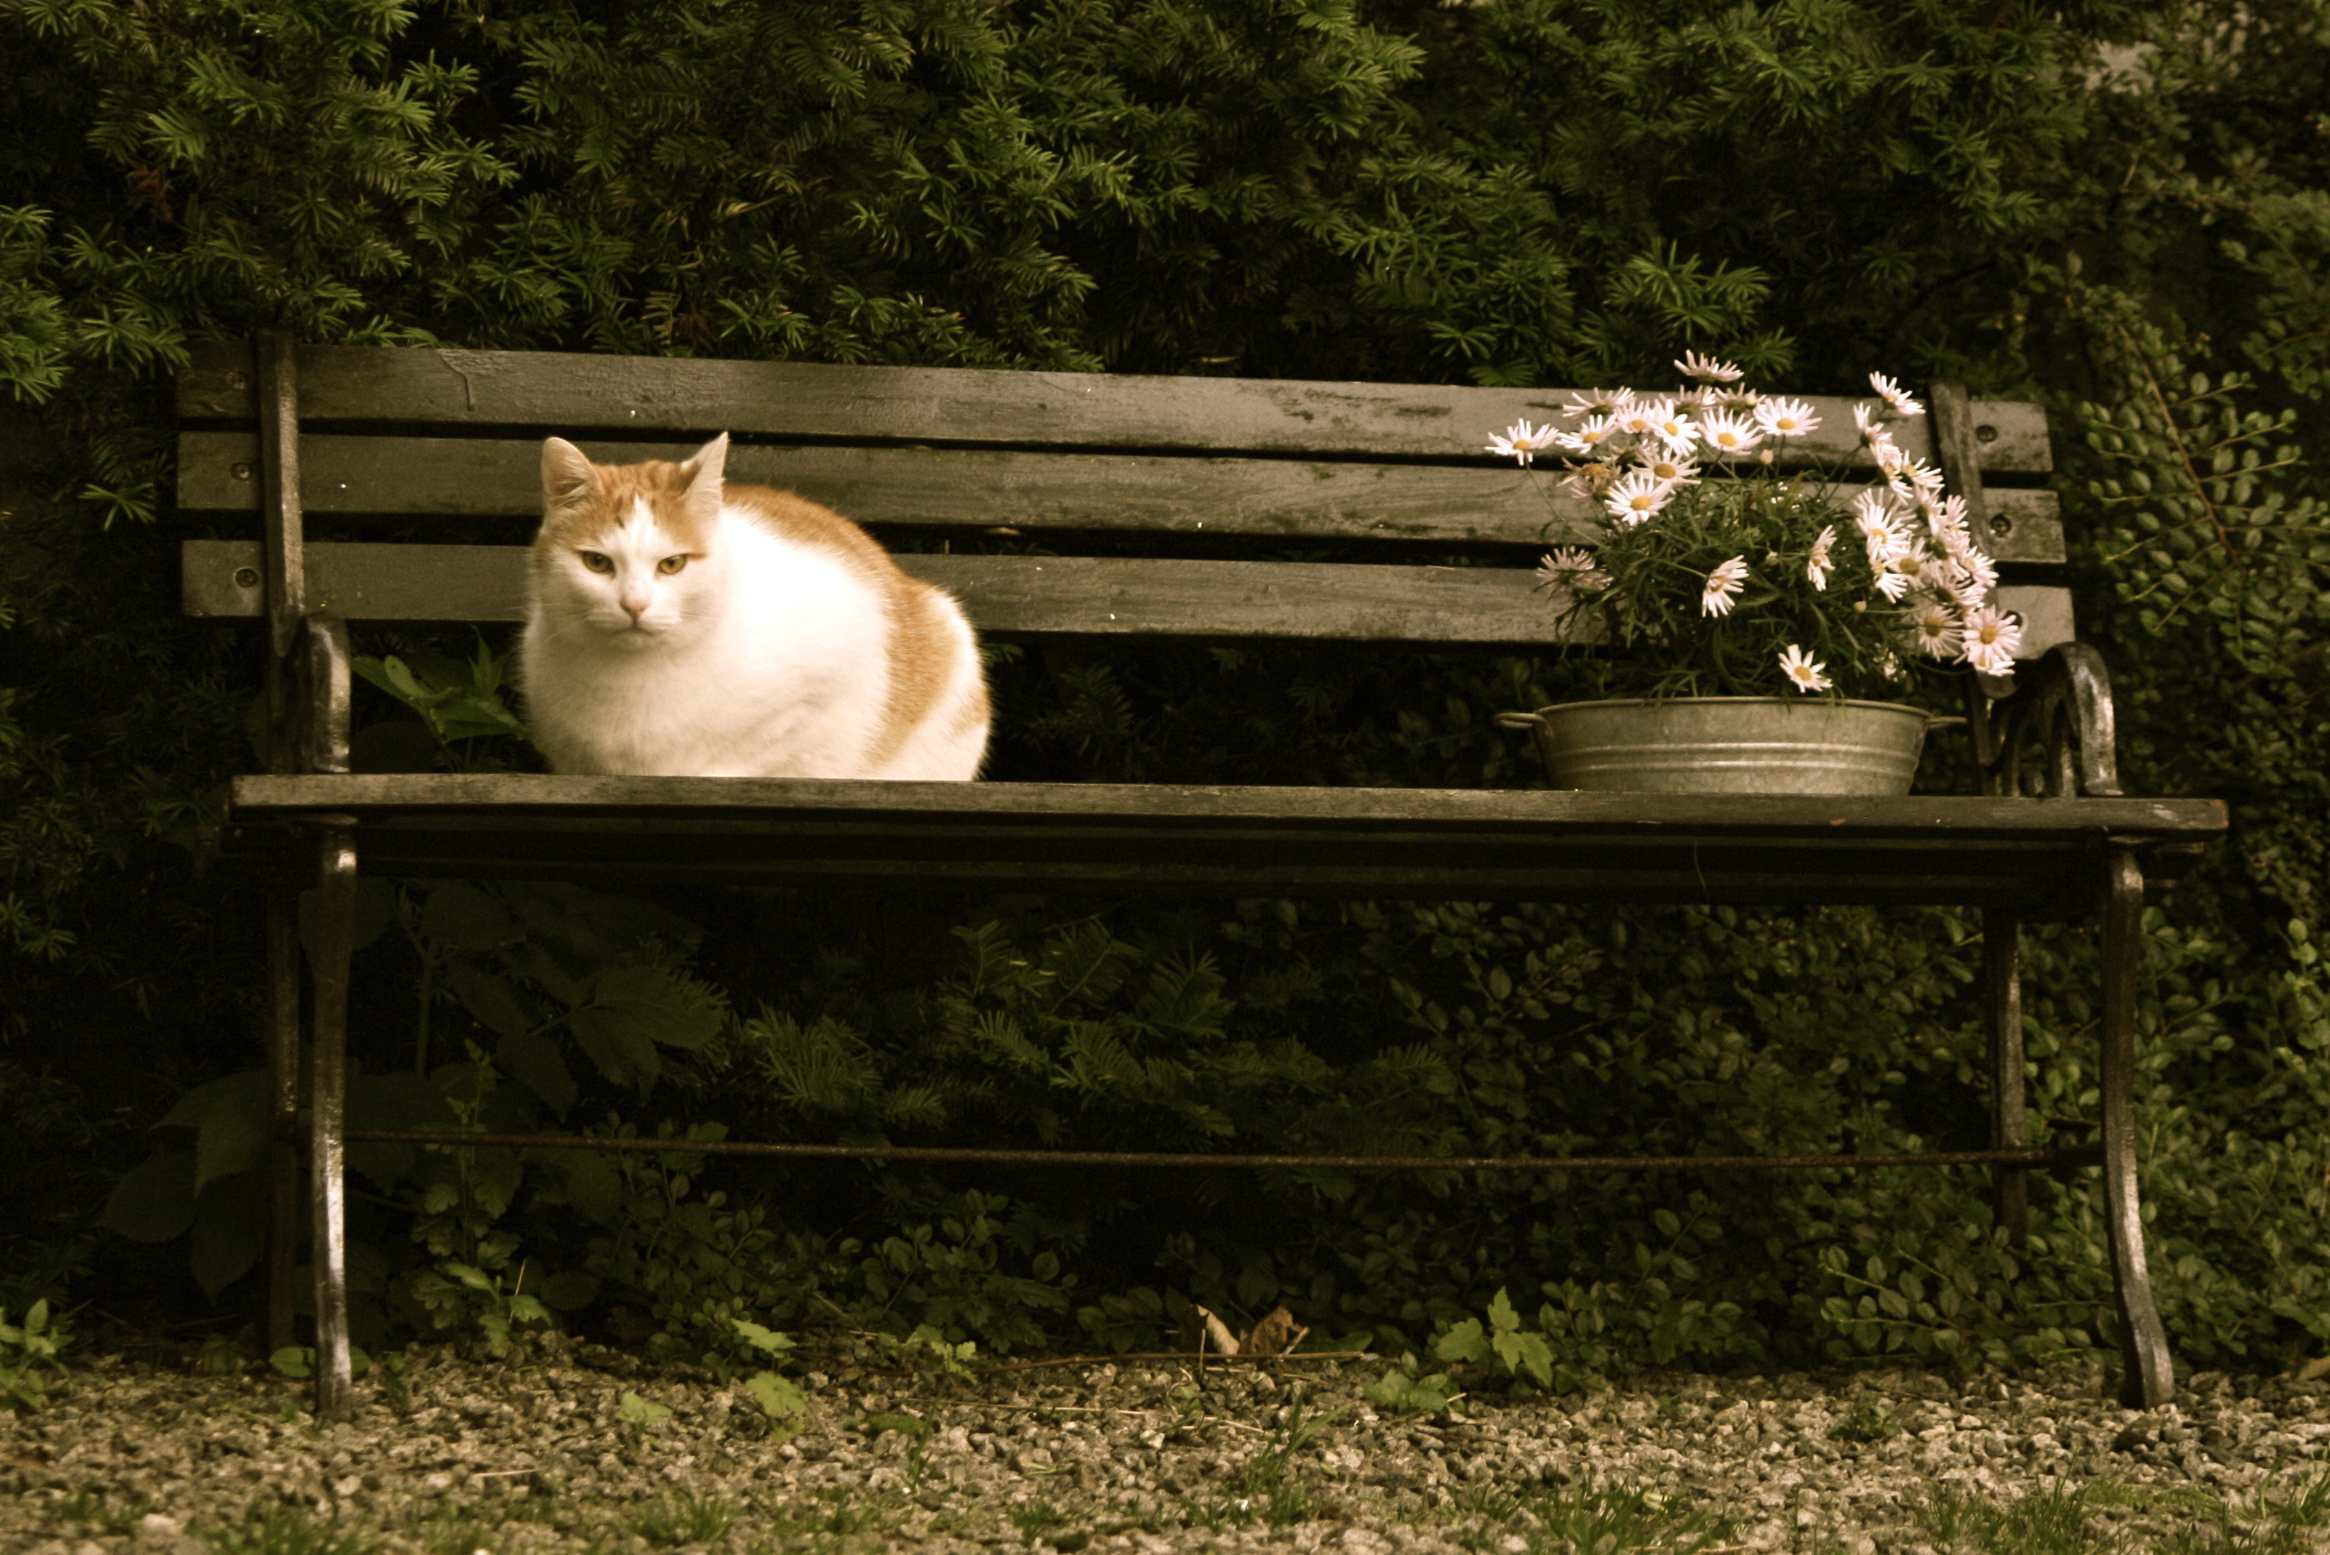
\includegraphics[scale=0.03]{./Figures/cat.jpg} $\rightarrow$ 
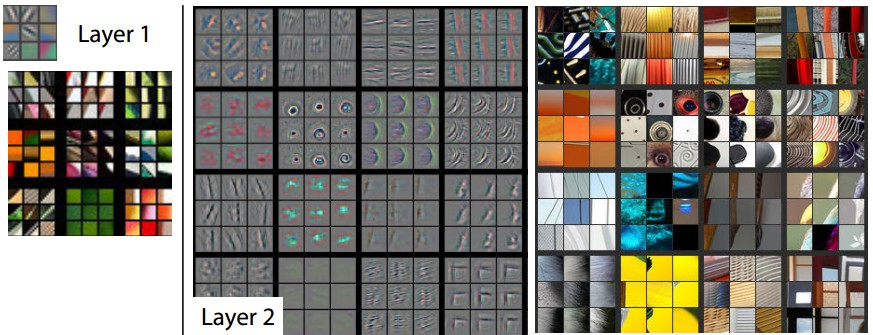
\includegraphics[scale=0.25]{./Figures/mattfeatures.jpeg}\\
\centering
$\downarrow$\\
$[\mbox{Third Layer Features}]$\\
$\downarrow$ \\
$\cdots$\\ 
$\downarrow$\\
\centering
$[\mbox{objects, orientations, positions, lighting, etc.}]$\\ \vspace{1.75cm} 
\emph{\tiny{Zeiler and Fergus. ECCV 2014}}
\end{frame} 

\begin{frame} 
\frametitle{Desirable Properties of Features}
\underline{Unsupervised Learning Problem:} \emph{Implicitly} learn features that facilitate solving \emph{many} problems simultaneously \\ \vspace{0.125cm}
\underline{Approach:} guess useful properties of features, then experimentally validate their usefulness on multiple problems
\begin{itemize}
\item{Informativeness $\rightarrow$ reconstruction, max-likelihood}
\item{Independence $\rightarrow$ Independent Component Analysis, Sparsity}
\item{Invariance $\rightarrow$ metric learning, Slow Feature Analysis, classifiers}
\item{Equivariance $\rightarrow$ linearization of transformations} 
\end{itemize} 
\end{frame} 

\begin{frame} 
\frametitle{Sparse Features - Informativeness, Independence}
\begin{center} 
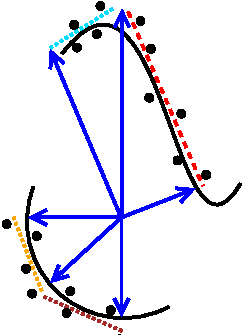
\includegraphics[scale=0.6]{./Figures/sparse2.pdf} \hspace{0.2cm}
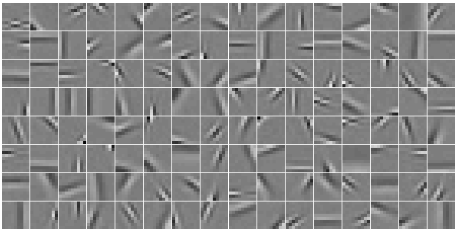
\includegraphics[scale=0.30]{./Figures/sparse_filters.png}
\end{center} 
\begin{eqnarray}
\nonumber 
L(x,W_e,W_d)= \sum_{i} \left(\underbrace{\|W_d ReLU(W_e x_i) - x_i\|^2}_{Reconstruction} +  \alpha \underbrace{ReLU(W_e x_i)}_{Sparsity} \right)
\end{eqnarray}
\begin{itemize} 
\item{Learns an over-complete basis which reconstructs the data by linearly combining a small subset of the available elements}
\item{Represents a local-linear model of the data manifold}
\item{Features are roughly independent}
\item{Highly unstable representation}
\end{itemize} 
\end{frame} 

\begin{frame} 
\frametitle{Similarity Metric Learning - Invariance}
\centering
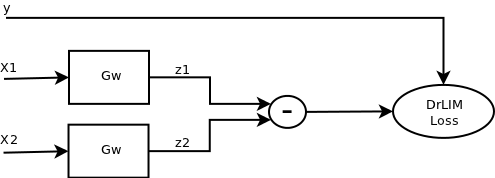
\includegraphics[scale=0.4]{./Figures/drlim_diag.png}
\begin{equation} 
\nonumber
L(x_i,x_j,W)=\left\{
                \begin{array}{ll}
                 \|G_W(x_i) - G_W(x_{j})\|_p, &\text{if $i$ similar to $j$}  \\
                 \max(0,m-\|G_W(x_i) - G_W(x_{j})\|_p) &\text{if $i$ dissimilar to $j$}
                \end{array}
              \right.
\end{equation} 
\begin{columns}[T] % align columns
\begin{column}{.6\textwidth}
\begin{itemize} 
\item{Global structure can be learned via local (stochastic) comparisons}
\item{Repulsive term does not guarantee informative features (low-dimensional visualization)} 
\item{$G_w()$ is the learned representation}   
\end{itemize} 
\emph{\tiny{Hadsell et al. CVPR 2006}}
\end{column}%
\begin{column}{.4\textwidth}
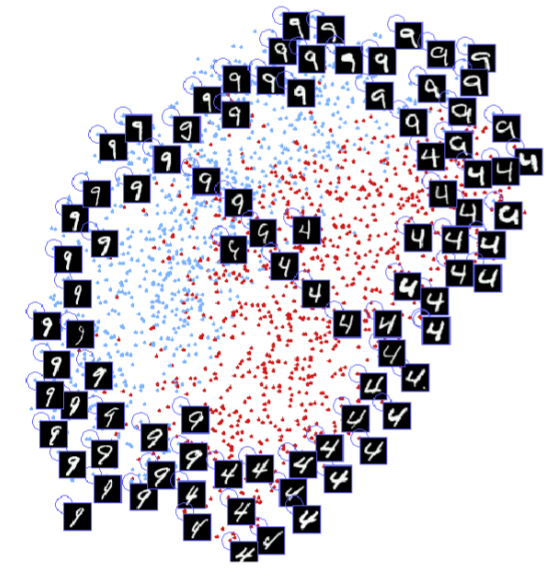
\includegraphics[scale=0.2]{./Figures/mnist.png}
\end{column}
\end{columns}
\end{frame}

\begin{frame}
\begin{center} 
\huge \color{blue} \emph{Unsupervised Learning from Video}
\end{center} 
\end{frame} 

\begin{frame} 
\frametitle{The Role of Time}
\begin{center} 
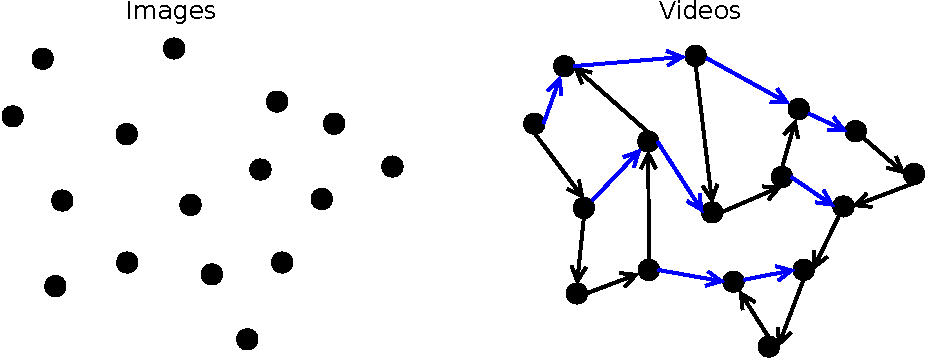
\includegraphics[scale=0.4]{./Figures/time.pdf}
\end{center} 
\begin{itemize} 
\item{Temporal sequences reveal neighbors in the \emph{latent} space}
\item{Natural videos are one-dimensional trajectories on the natural image manifold}
\item{Time shows you who your neighbors are}
\end{itemize} 
\end{frame} 

\begin{frame} 
\frametitle{Toy Example 1}
\begin{center} 
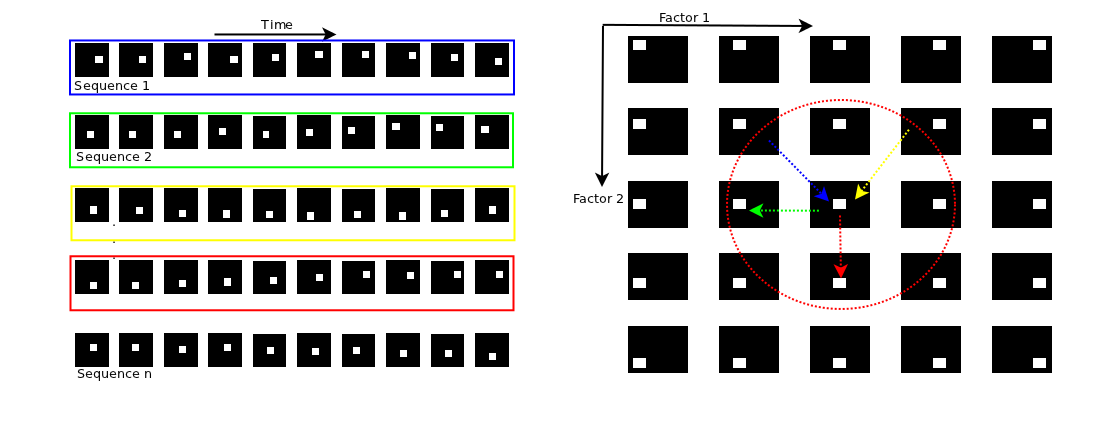
\includegraphics[scale=0.25]{./Figures/toy_video.png}
\end{center} 
\begin{itemize} 
\item{Consider video sequences of a single pixel moving with \emph{no overlap between successive frames}}
\item{Extrinsic measures (e.g. $L^2$) of similarity are useless}
\end{itemize} 
\end{frame} 

\begin{frame} 
\frametitle{Toy Example 2}
\begin{columns}[T] % align columns
\begin{column}{.5\textwidth}
DrLIM learns intrinsic factors of variation when trained on video \\ \vspace{0.25cm} 
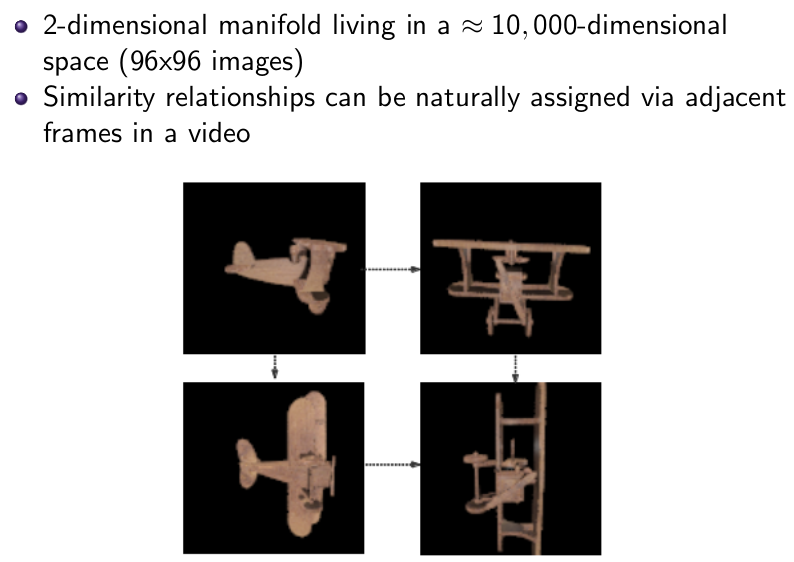
\includegraphics[scale=0.20]{./Figures/drlim_data.png} 
\begin{itemize} \tiny \item{Learning features that decrease the variability between temporally adjacent samples are known as ``slow features''} 
\tiny \item{Without additional constraints slow features collapse to constants}
\end{itemize} 
\end{column} 
\begin{column}{.5\textwidth}
\hspace{0.25cm} \tiny{Color-map Yaw} \hspace{0.8cm} \tiny{Color-map Roll} \\
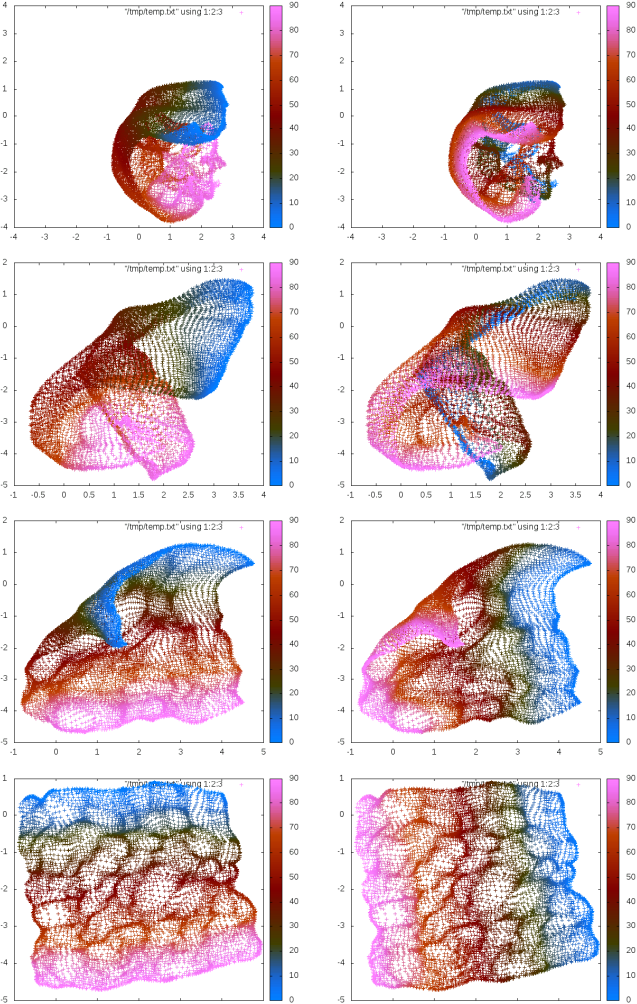
\includegraphics[scale=0.20]{./Figures/drlim.png}
\end{column}
\end{columns}
\end{frame} 

\begin{frame}
\begin{center} 
\huge \color{blue} \emph{Unsupervised Learning of Spatiotemporally Coherent Metrics}
\end{center} 
\end{frame}

\begin{frame}
\frametitle{The Model}
\underline{Description:} Sparse auto-encoder whose activations are $L^2$-pooled in local groups, on which slowness regularization is applied.
\begin{center} 
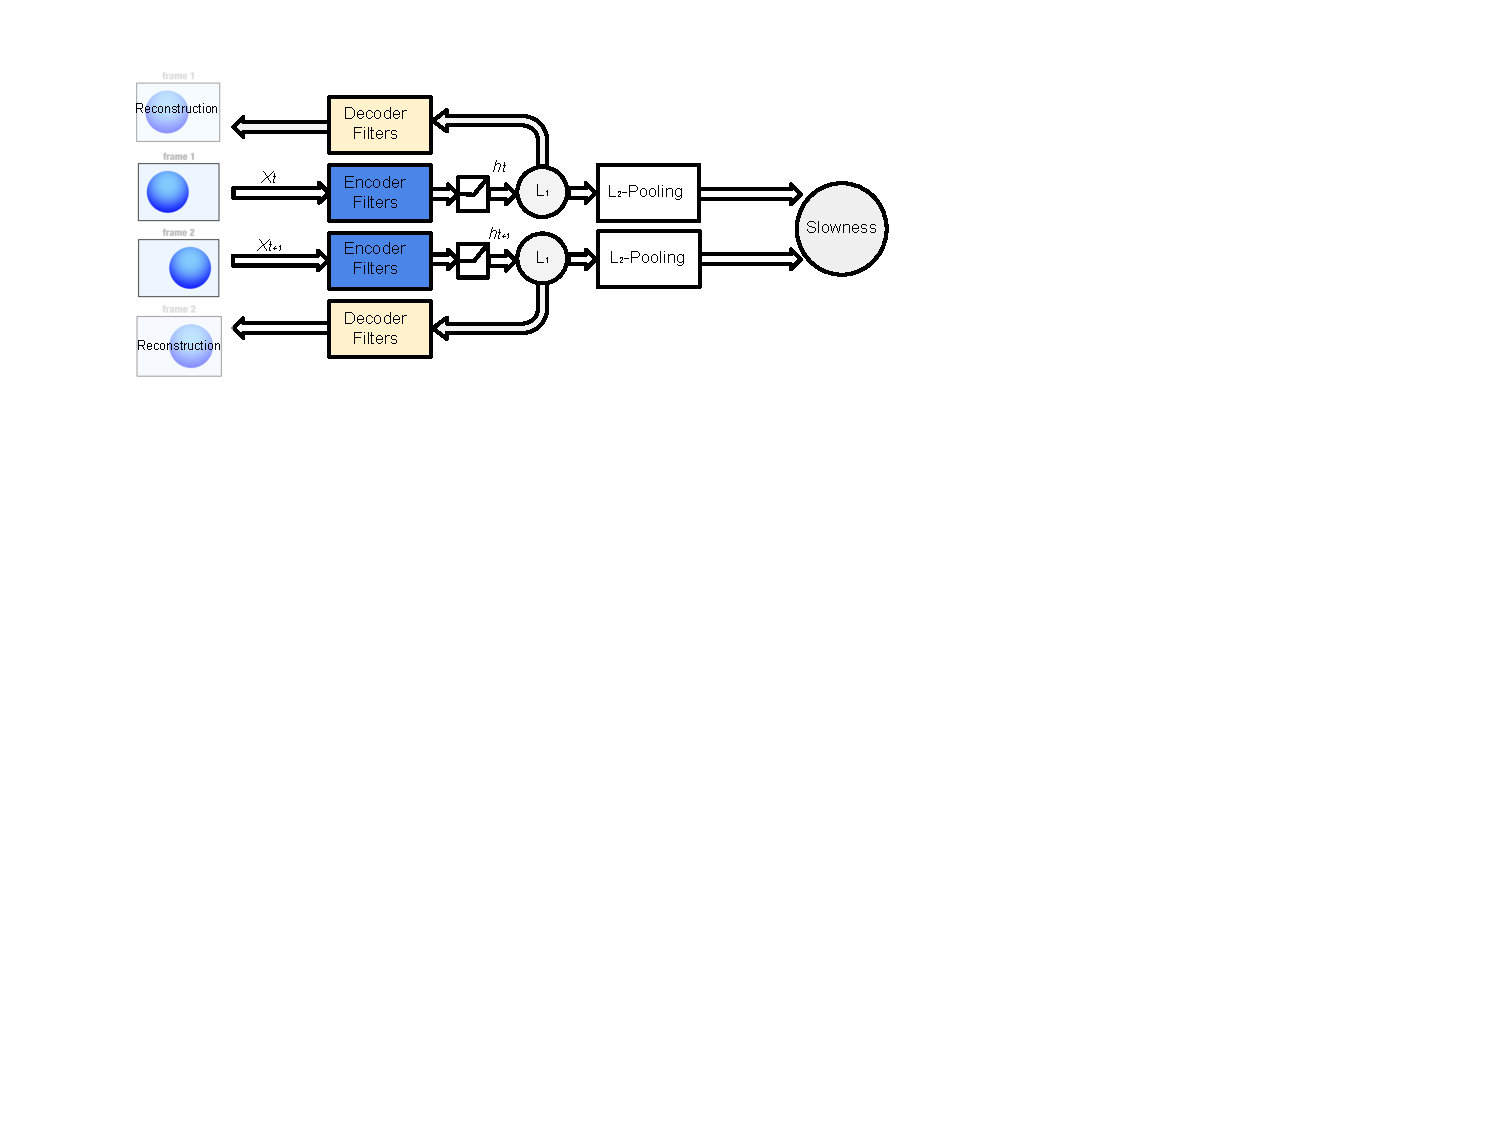
\includegraphics[scale=0.50,trim = 15 350 290 39, clip]{./Figures/Project1/diagram.pdf} \\
{\small
\begin{eqnarray}
\nonumber 
L(x_t,x_{t'},W_e,W_d)= \sum_{\tau = \{t,t'\}} \left(\underbrace{\|W_d ReLU(W_e x_\tau) - x_\tau\|}_{\mbox{\tiny Reconstruction}} +  \alpha \underbrace{ReLU(W_e x_\tau)}_{\mbox{\tiny Sparsity}} \right) \\
\nonumber
 + \underbrace{\beta \sum_{i=1}^K \left| \|ReLU(W_ex_t)\|^{P_i} - \|ReLU(W_ex_{t'})\|^{P_i} \right|}_{\mbox{\tiny Slowness after local $L^2$ pooling}}
\end{eqnarray}}
\end{center} 
\end{frame} 

\begin{frame}
\frametitle{Intuitive Interpretation}
\centering
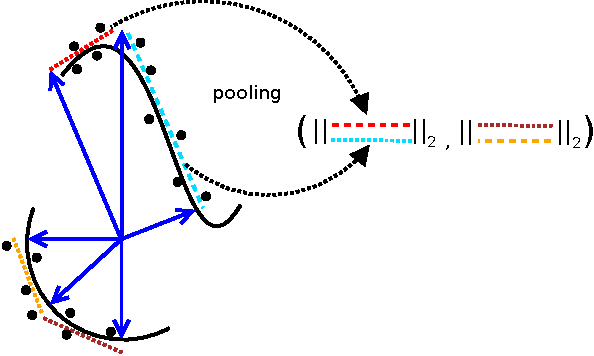
\includegraphics[scale=0.65]{./Figures/SF2.pdf} \\
\begin{itemize} 
\item{\underline{Reconstruction} $\rightarrow$ promotes informative features}
\item{\underline{Sparsity} $\rightarrow$ promotes independent features}
\item{\underline{Slowness} $\rightarrow$ promotes invariant features}
\end{itemize} 
\end{frame} 

\begin{frame}
\frametitle{Fourier Interpretation}
$\rightarrow$ Fully connected features learned by training on natural videos patches mainly learn (local) \emph{translation invariance} \\
$\rightarrow$ Train convolutional features to learn a richer class of invariants
\begin{center} 
\begin{figure}
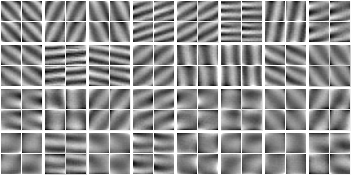
\includegraphics[scale=0.38]{./Figures/Project1/slow_dec_pooling_sub.png}
\caption{Without sparsity, $\alpha = 0$}
\end{figure} 
\begin{figure}
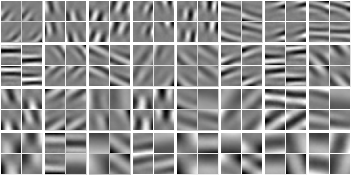
\includegraphics[scale=0.38]{./Figures/Project1/slow_dec_l1_pooling.png}
\caption{With sparsity, $\alpha > 0$}
\end{figure} 
\end{center} 
\end{frame} 

\begin{frame}
\frametitle{Dataset and Hyper-Parameter Selection}
\underline{Problem:} what is the correct trade-off between informativeness and invariance for natural data? In other words, how do we set the hyper-parameters $\alpha$ and $\beta$ without supervision? 
\begin{center} 
\begin{figure}
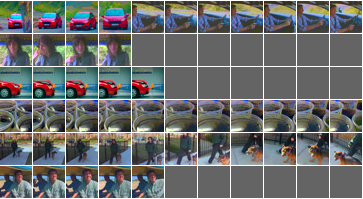
\includegraphics[scale=0.40]{./Figures/Project1/youtube.png}
\caption{Weakly segmented scenes from our YouTube dataset}
\end{figure}
\end{center}
\underline{Temporally Coherent Feature Space:} a feature space which induces the nearest neighbors to be the temporal neighbors (temporal invariance)   
\end{frame} 

\begin{frame}
\frametitle{Visualizing Temporal Coherence - YouTube}
\begin{center} 
\begin{figure}
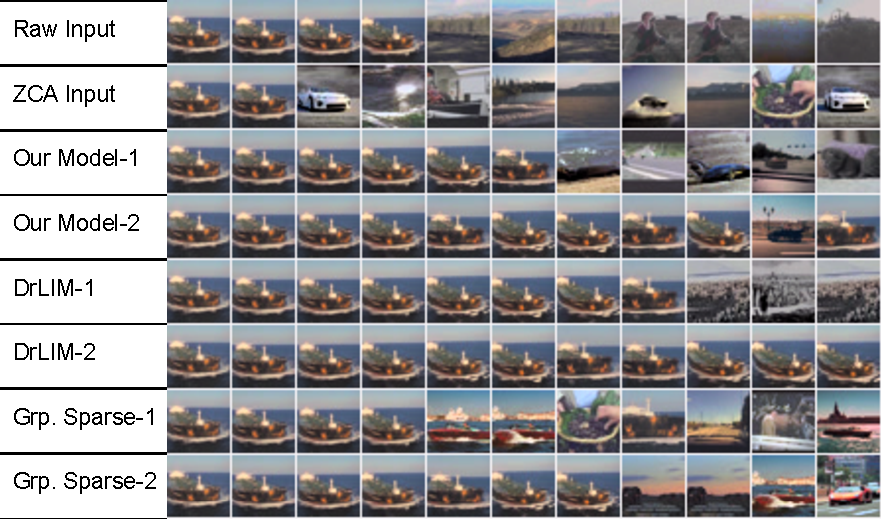
\includegraphics[scale=0.40]{./Figures/Project1/NNtime1.pdf}\\ \vspace{0.25cm} 
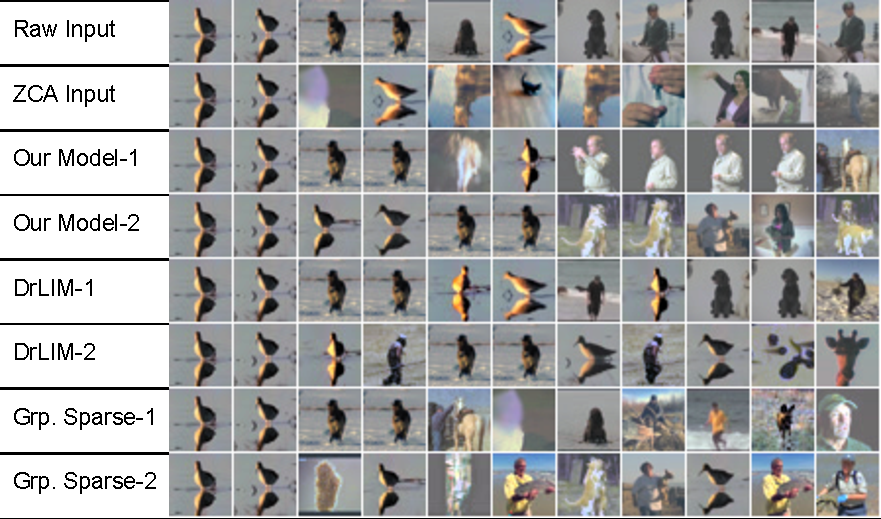
\includegraphics[scale=0.40]{./Figures/Project1/NNtime2.pdf}
\end{figure}
\end{center}  
\end{frame} 

\begin{frame}
\frametitle{Convolutional $1^{st}$ Layer Features}
\begin{center} 
\begin{figure} 
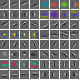
\includegraphics[scale=1.5]{./Figures/Project1/filters_slow.png} \hspace{0.5cm} 
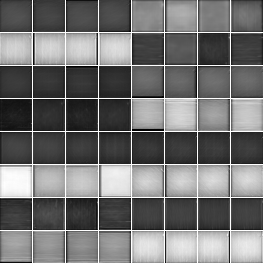
\includegraphics[scale=0.45]{./Figures/Project1/act_large_slow.png}
\end{figure} 
\end{center} 
\underline{Left:} Activations are pooled \emph{across feature maps} in non-overlapping groups of four \\
\underline{Right:} Activation frequency for corresponding feature over entire dataset
\end{frame} 

\begin{frame}
\frametitle{Visualizing Semantic Coherence - CIFAR10}
\begin{center} 
\begin{figure}
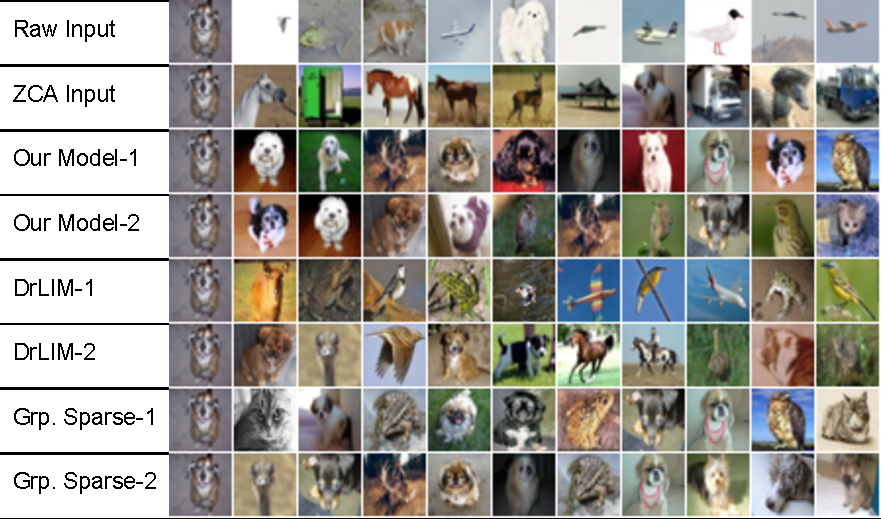
\includegraphics[scale=0.40]{./Figures/Project1/NNclass1.pdf}\\ \vspace{0.25cm} 
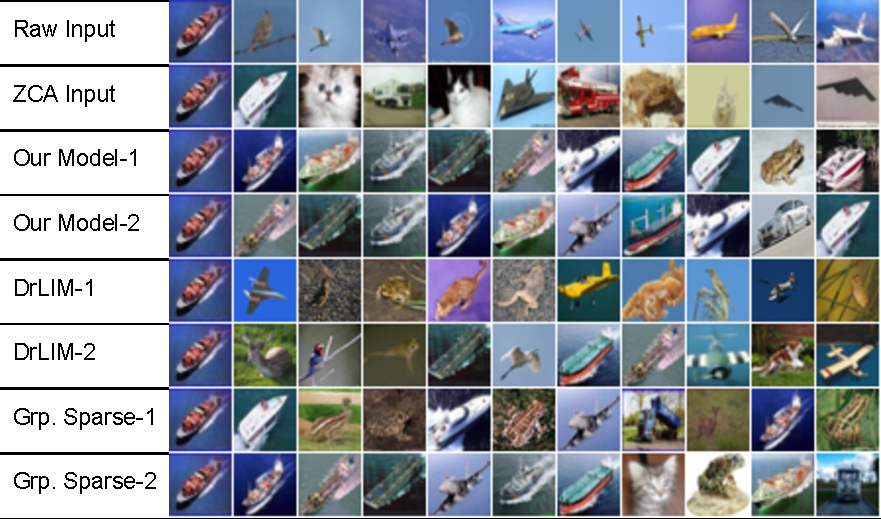
\includegraphics[scale=0.40]{./Figures/Project1/NNclass2.pdf}
\end{figure}
\end{center}  
\end{frame} 

\begin{frame}
\frametitle{Precision-Recall}
\begin{center} 
\begin{figure}
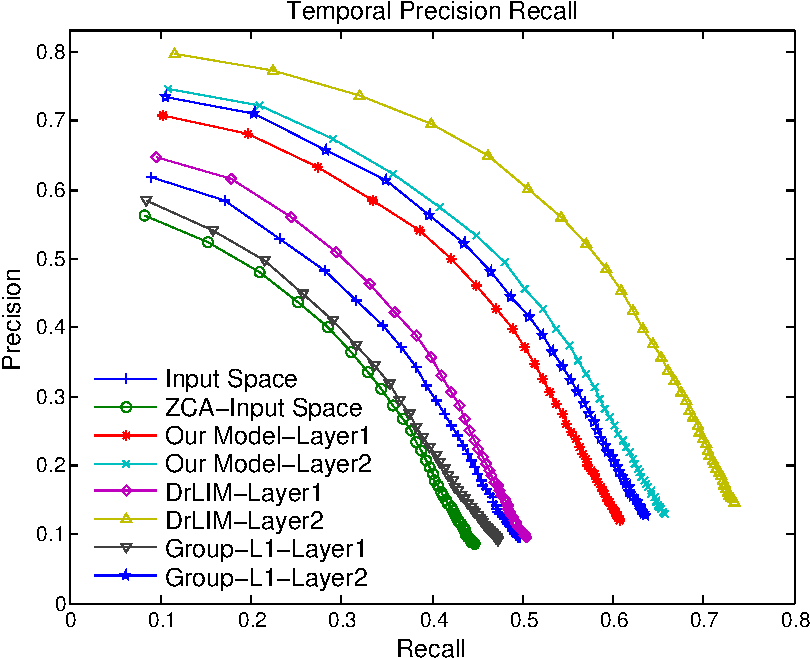
\includegraphics[scale=0.40]{./Figures/Project1/AUC_time-crop.pdf}
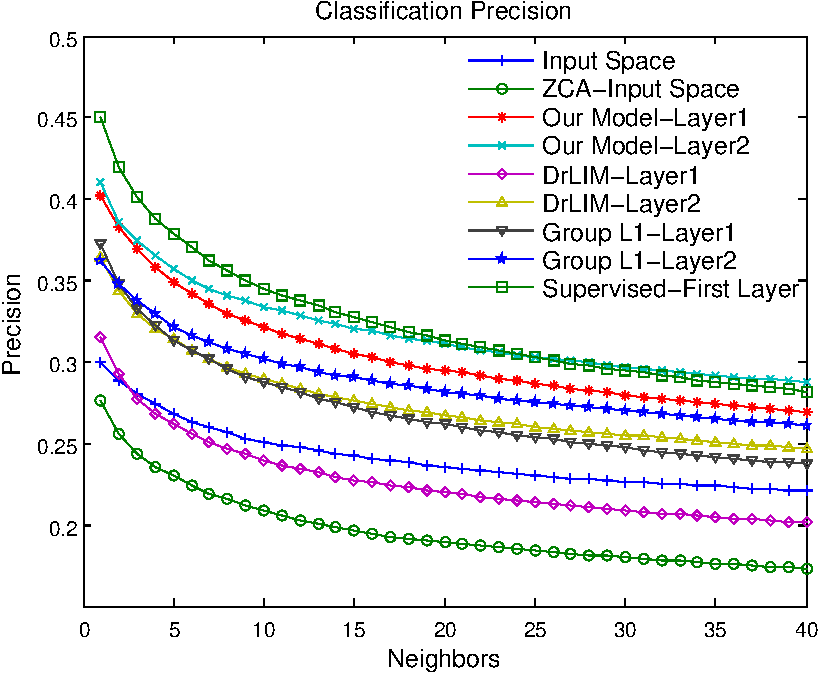
\includegraphics[scale=0.40]{./Figures/Project1/AUC_class-crop.pdf} 
\caption{\underline{Temporal PR:} Percent of nearest neighbors from the same \textbf{\emph{scene}} \\
\hspace{1.15cm}\underline{Class PR:} Percent of nearest neighbors from the same \textbf{\emph{class}} }
\end{figure}
\end{center}  
\end{frame} 

\begin{frame}
\frametitle{Correlation between Temporal and Class AUCs}
\centering
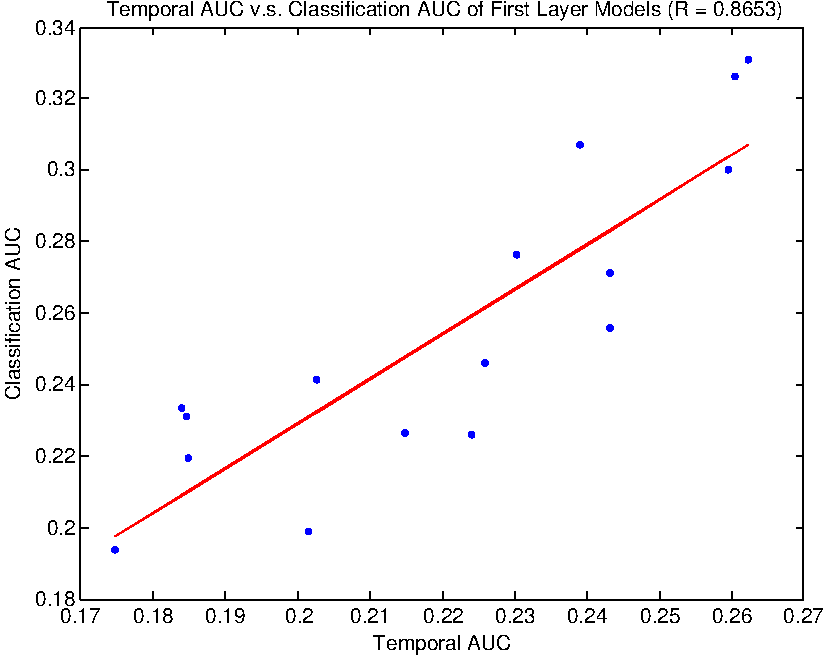
\includegraphics[scale=0.5]{./Figures/Project1/scatter-crop.pdf}\\
This demonstrates that a \emph{semantically} coherent metric can be learned implicitly by maximizing \emph{temporal coherence}.  
\end{frame} 

\begin{frame}
\frametitle{Shortcomings}
\begin{itemize}
\item{Layer-wise greedy training} 
\item{Too many hyper-parameters require costly optimization} 
\item{Partial reconstruction means that the final features may have lost information}
\end{itemize} 
\end{frame} 

\begin{frame}
\begin{center} 
\huge \color{blue} \emph{Learning to Linearize under Uncertainty}
\end{center} 
\end{frame}

\begin{frame} 
\frametitle{Features that Linearize Temporal Trajectories}
\begin{center} 
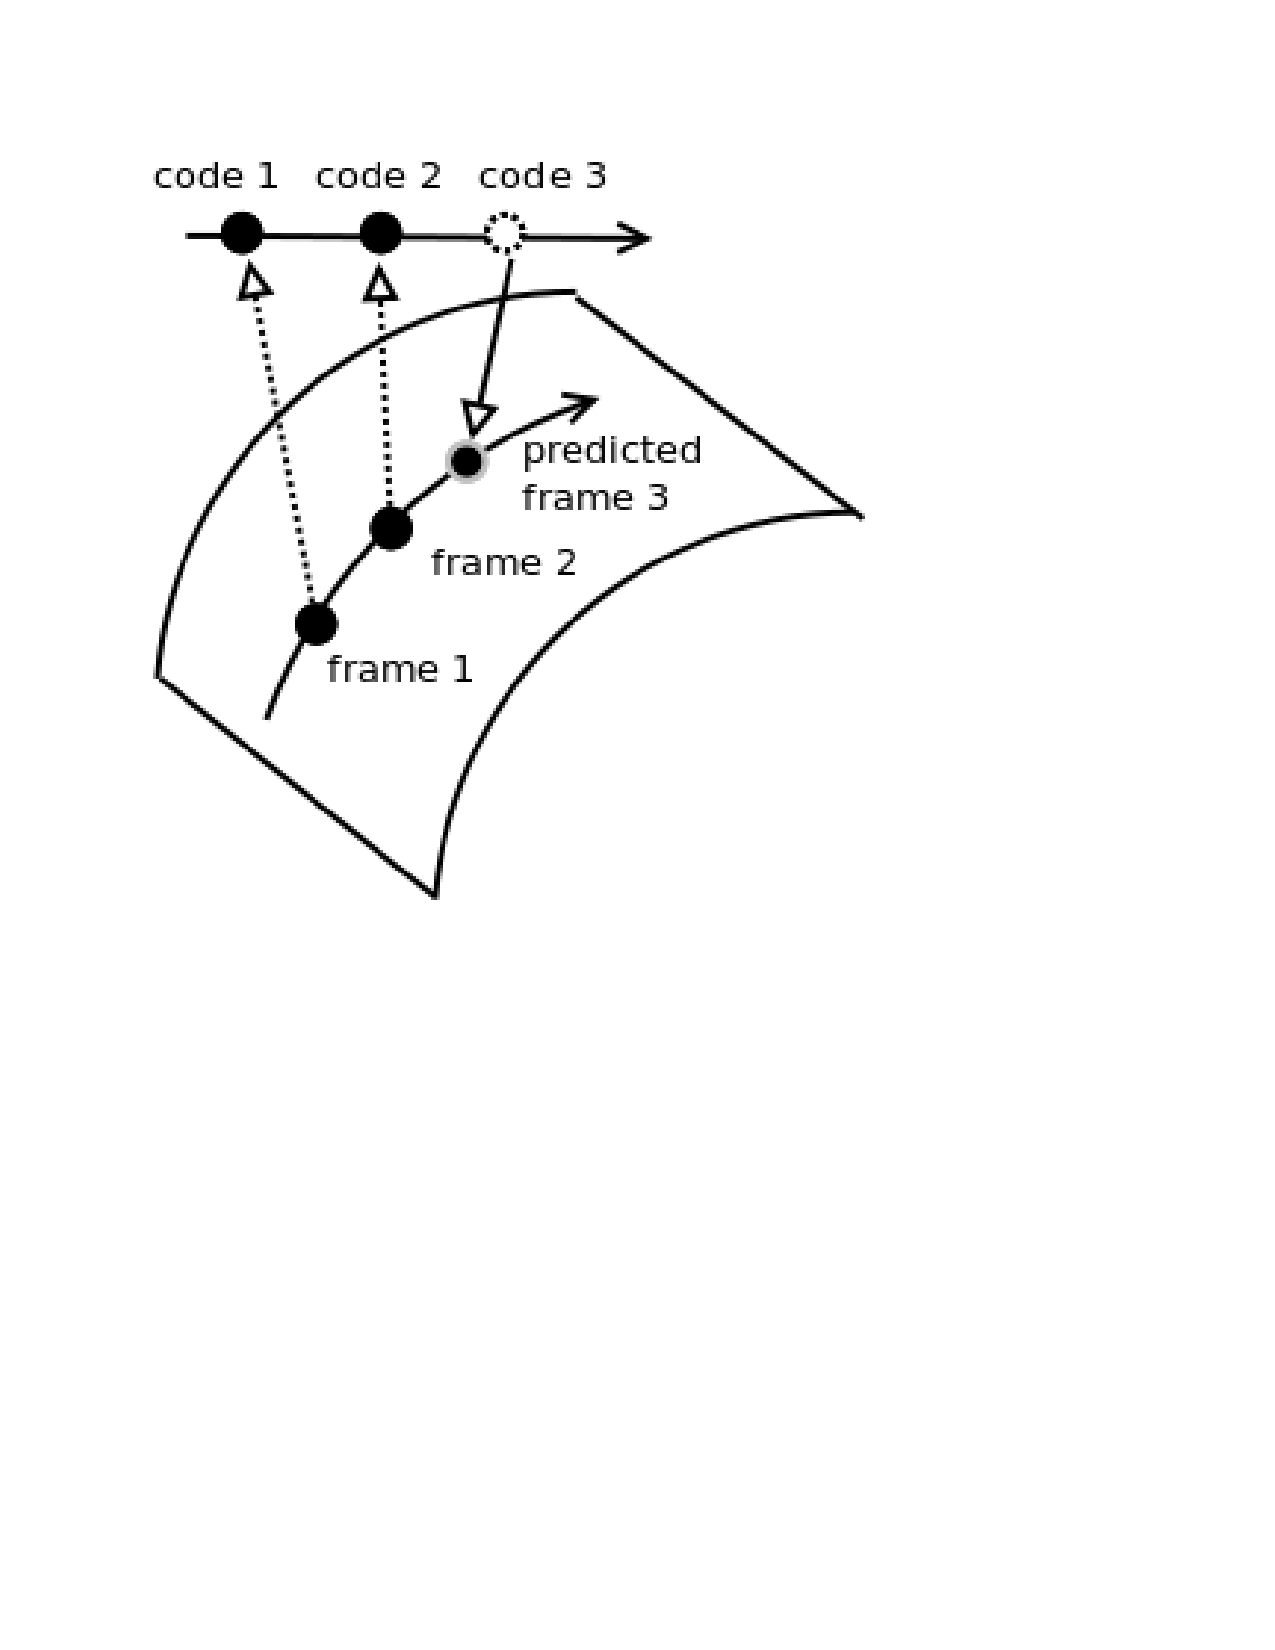
\includegraphics[scale=0.27, trim= 15 350 200 39, clip]{./Figures/Project2/linearize_manifold.pdf} 
\end{center} 
Let $X = \{...,x^{t-1},x^t,x^{t+1},...\}$ be a sequence of frames and denote the code for frame $x^t$ by $z^t = F_W(x^t)$, 
where $F_W()$ and $G_W()$ denote the encoder and decoder, respectively. \\
\begin{equation}
\nonumber
L = \frac{1}{2}\| G_W(\mathbf [2 ~~-1] \begin{bmatrix}z^t&z^{t-1}\end{bmatrix}^T) - x^{t+1} \|^2_2
\label{eqn:loss} 
\end{equation} 
\vspace{0.430cm} 
\end{frame} 

\begin{frame} 
\frametitle{Features that Linearize Temporal Trajectories}
\begin{center} 
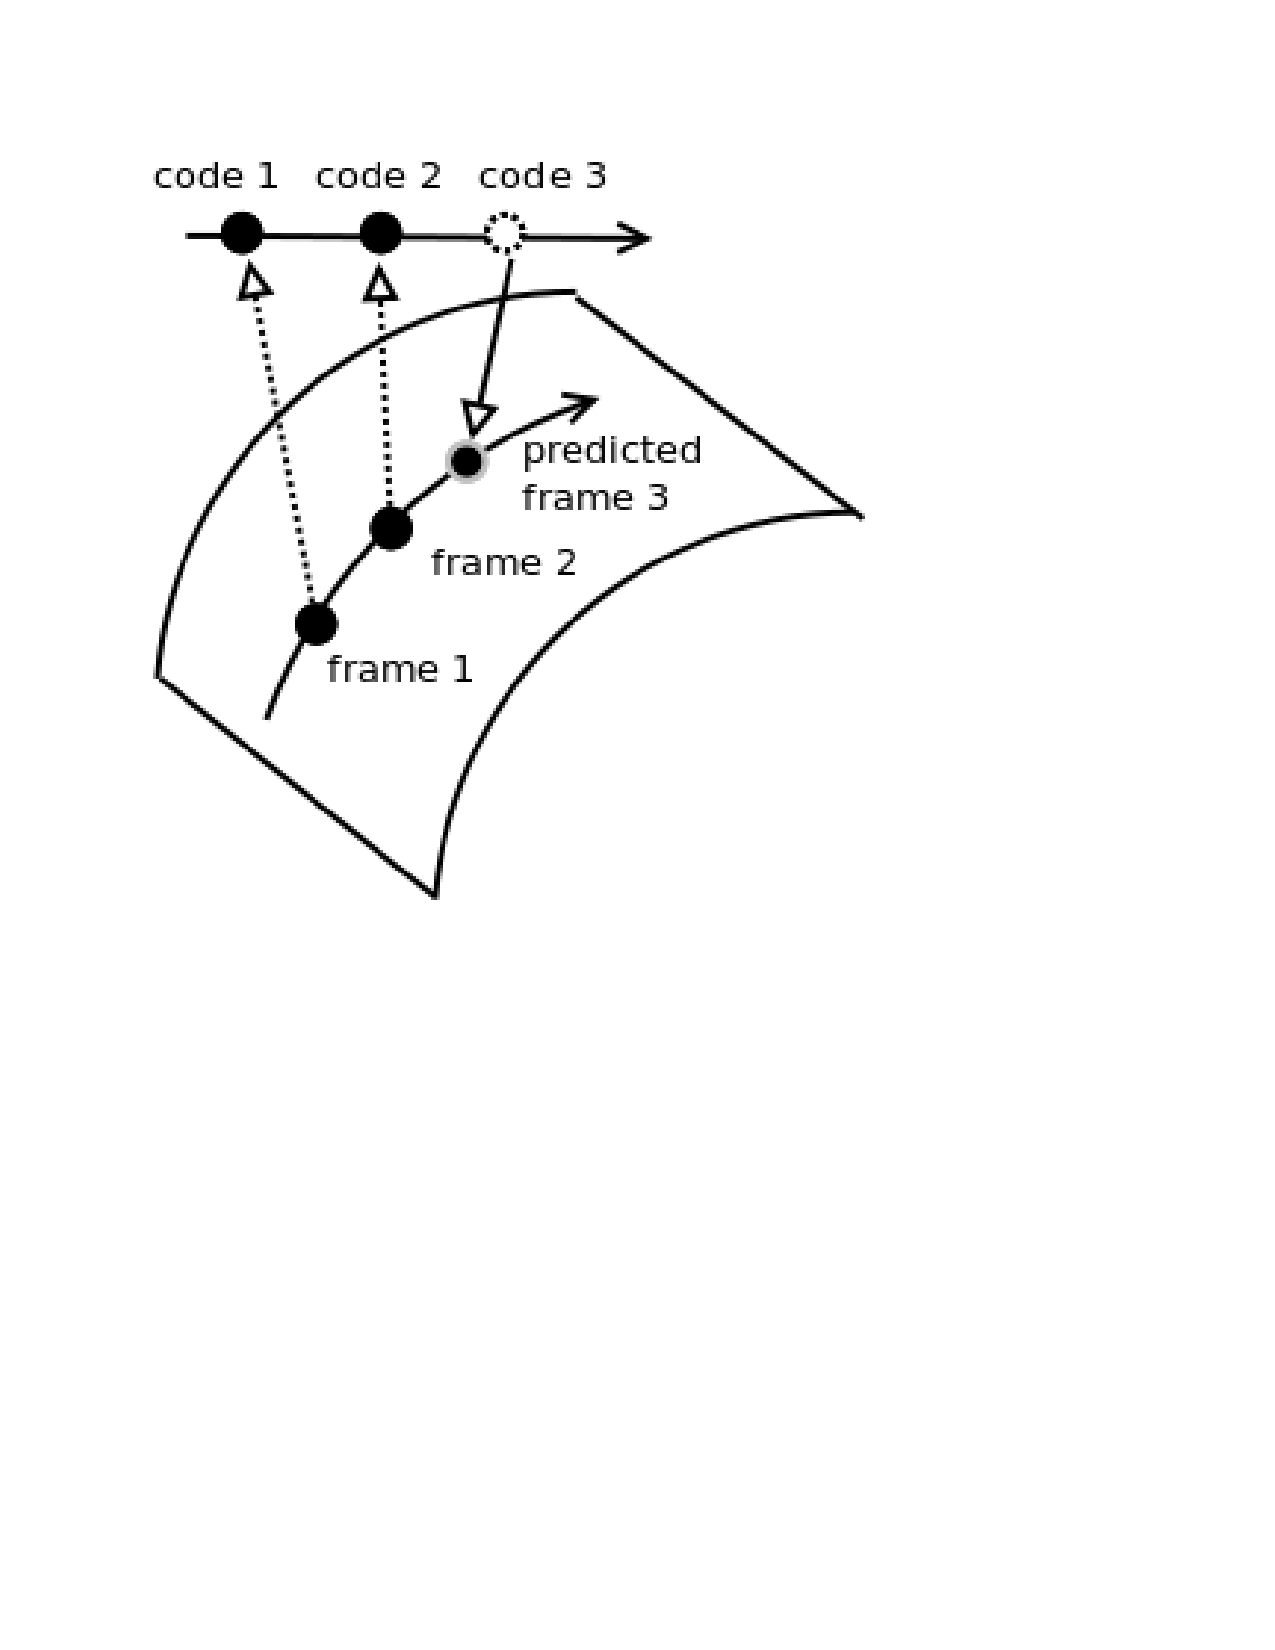
\includegraphics[scale=0.27, trim= 15 350 200 39, clip]{./Figures/Project2/linearize_manifold.pdf} 
\end{center} 
Let $X = \{...,x^{t-1},x^t,x^{t+1},...\}$ be a sequence of frames and denote the code for frame $x^t$ by $z^t = F_W(x^t)$, 
where $F_W()$ and $G_W()$ denote the encoder and decoder, respectively. \\
\begin{equation}
\nonumber
L = \frac{1}{2}\| G_W(\mathbf [2 ~~-1] \begin{bmatrix}z^t&z^{t-1}\end{bmatrix}^T) - x^{t+1} \|^2_2 - \lambda \frac{(z^t - z^{t-1})^T(z^{t+1} - z^t)}{\|z^t-z^{t-1}\| \|z^{t+1} - z^t\|}
\label{eqn:loss} 
\end{equation} 
\end{frame} 

\begin{frame} 
\frametitle{Toy Example: 3-Pixel Movie}
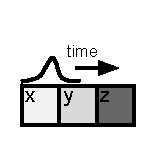
\includegraphics[scale=1]{./Figures/Project2/fig1.pdf} 
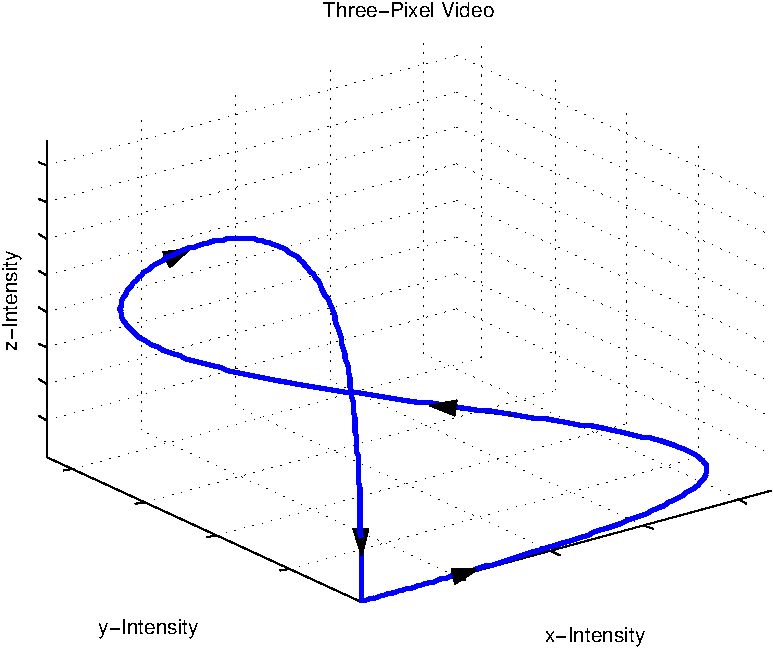
\includegraphics[scale=0.5]{./Figures/Project2/fig2.pdf} \\
\begin{center} 
What is the linearized feature of this data set? \\
\textbf{Implicitly learn to track common patterns in the image}
\end{center} 
\end{frame} 

\begin{frame} 
\frametitle{Phase-Pooling Operator}
\begin{itemize} 
\item{Define a soft version of the $max$ (``what'') and $argmax$ (``where'') operators applied to each pool group}
\end{itemize} 
\begin{equation}
\nonumber
m_k = \sum_{N_k} z(f,x,y)\!~ \frac{e^{\beta z(f,x,y)}}{\sum_{N_k}e^{\beta z(f\prime, x\prime, y\prime )}}\, \approx\underset{N_k}\max~z(f,x,y)
\label{eqn:mag}
\end{equation}
\begin{itemize} 
\item{Assuming that the activation pattern within each neighborhood is approximately unimodal}
\item{The vector $\mathbf p_k$ approximates the local coordinates in the feature topology at which the max activation value occurred}
\end{itemize} 
\begin{equation}
\nonumber
\mathbf p_k = \sum_{N_k}
\begin{bmatrix}
f \\ x \\ y
\end{bmatrix}
\frac{e^{\beta z(f,x,y)}}{\sum_{N_k}e^{\beta z(f\prime, x\prime, y\prime )}} \approx\underset{ N_k}\argmax~z(f,x,y)
\label{eqn:phase}
\end{equation}  
\begin{itemize} 
\item{We can now back-propagate through the location of the activation, i.e. the ``switch locations''}
\end{itemize} 
\end{frame} 

\begin{frame} 
\frametitle{Complete Architecture}
\begin{center}
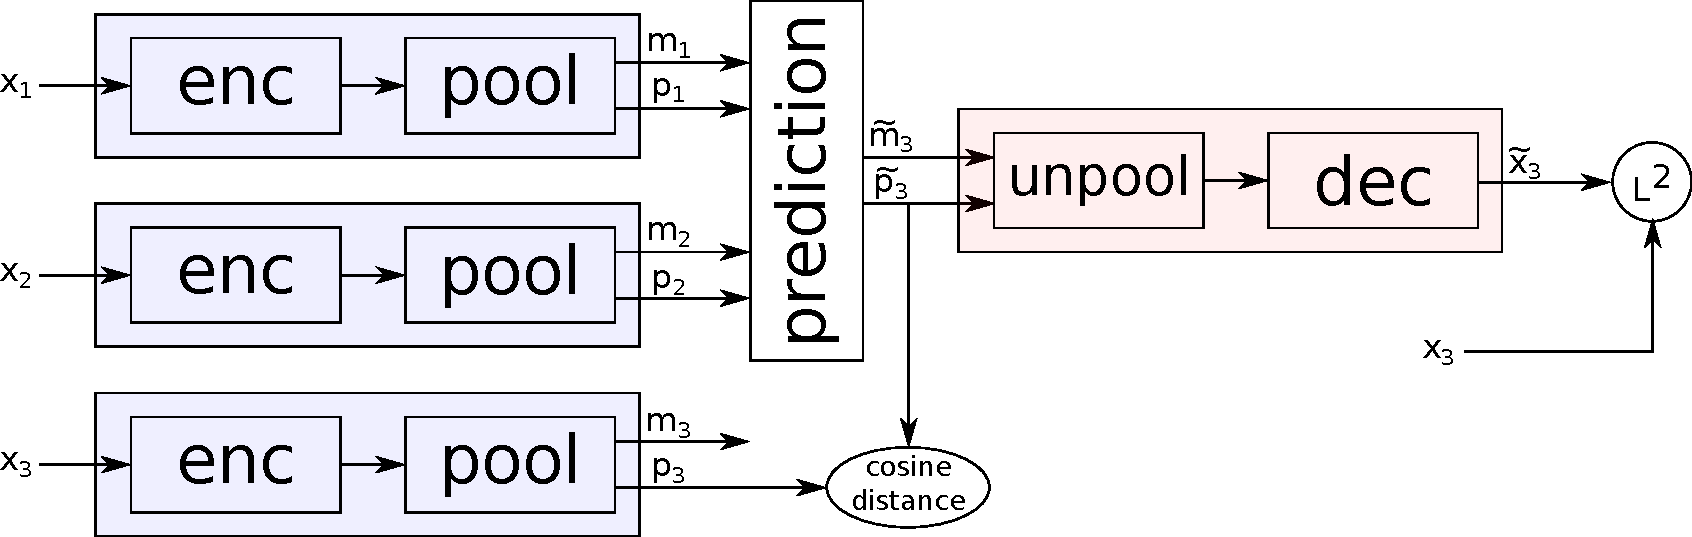
\includegraphics[scale=0.38]{./Figures/Project2/network.pdf}  
\end{center} 
The predicted magnitude and phase are defined as follows: 
\begin{eqnarray}
\nonumber
m^{t+1}=&\frac{m^t + m^{t-1}}{2}&\\
\label{eqn:magpred} 
\nonumber
\mathbf p^{t+1}=&2\mathbf p^t-\mathbf p^{t-1}& 
\label{eqn:phasepred} 
\end{eqnarray} 
Define an ``\emph{un-pooling}'' operation of the decoder that produces reconstructed activation maps by placing the magnitudes $m$ at appropriate locations given by the phases $\mathbf p$.
\end{frame} 

\begin{frame} 
\frametitle{Visualization of $1^{st}$-Layer Features}
\begin{center} 
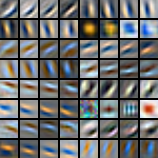
\includegraphics[scale=0.6]{./Figures/Project2/pretty_decoder.png} \hspace{1cm} 
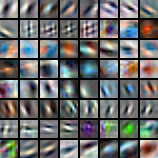
\includegraphics[scale=0.6]{./Figures/Project2/dec200.png} 
\end{center} 
\underline{Left:} Phase-pooling in non-overlapping groups (synthetic video) \\
\underline{Right:} Phase-pooling in overlapping groups (natural video) 
\end{frame} 

\begin{frame} 
\frametitle{Addressing Uncertainty}
\begin{itemize}
\item If multiple outcomes are present in the training set then minimizing the $L^2$ distance to these multiple outcomes induces the network to predict the \emph{average outcome} 
\item Introduce latent variables $\delta$ to the prediction architecture that are not deterministic functions of the input
\item The $\delta$-corrected code is defined as:
\begin{equation} 
\nonumber 
\label{eqn:delta}
\hat z^{t+1}_\delta =  z^{t} + (W_1 \delta) \odot [2~~-1]\begin{bmatrix}z^t&z^{t-1}\end{bmatrix}^T
\end{equation}  
\end{itemize}
\centering
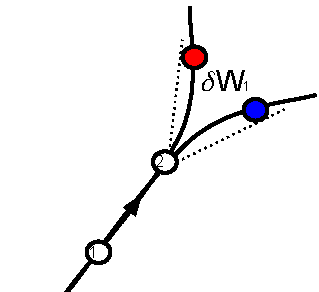
\includegraphics[scale=0.5]{./Figures/Project2/delta_ambiguity.pdf} \\
\end{frame} 

\begin{frame} 
\frametitle{Addressing Uncertainty}
The $\delta$-corrected loss is: 
\begin{equation} 
\nonumber 
\label{eqn:delta_loss}
L = \min\limits_\delta \| G_W(\hat z_\delta ^{t+1}) - x^{t+1} \|^2_2 - \lambda \frac{(z^t - z^{t-1})^T(z^{t+1} - z^t)}{\|z^t-z^{t-1}\| \|z^{t+1} - z^t\|} 
\end{equation} 
\end{frame} 

\begin{frame}  
\frametitle{Architectures}
\begin{table} 
\begin{tiny}
\centering
\resizebox{\linewidth}{!}{
\begin{tabular}{| c | c | c | c | }
	\hline
    & Encoder & Prediction & Decoder \\
    \hline
    \multirow{2}{*}{Shallow Architecture 1} &
    Conv+ReLU $64\times9\times9$ &
    Average Mag. &
    \multirow{2}{*}{Conv $64\times9\times9$} \\
    & Phase Pool 4 & Linear Extrap. Phase & \\
    \hline
    \multirow{2}{*}{Shallow Architecture 2} &
    Conv+ReLU $64\times9\times9$ &
    Average Mag. &
    \multirow{2}{*}{Conv $64\times9\times9$} \\
    & Phase Pool 4 stride 2 &
    Linear Extrap. Phase & \\
    \hline
    \multirow{6}{*}{Deep Architecture 1} &
    & \multirow{6}{*}{None} &
    FC+ReLU $\mathbf{8192}\times8192$\\
    &Conv+ReLU $16\times9\times9$ & &
    Reshape $32\times16\times16$\\
    &Conv+ReLU $32\times9\times9$ & &
    SpatialPadding $8\times8$ \\
    &FC+ReLU $8192\times4096$ & &
    Conv+ReLU $16\times9\times9$\\
    &&&SpatialPadding $8\times8$\\
    &&&Conv $1\times9\times9$ \\
    \hline
    \multirow{6}{*}{Deep Architecture 2} &
    &\multirow{6}{*}{Linear Extrapolation}&
    FC+ReLU $4096\times8192$\\
    & Conv+ReLU $16\times9\times9$ & &
    Reshape $32\times16\times16$\\
    &Conv+ReLU $32\times9\times9$ &&
    SpatialPadding $8\times8$\\
    &FC+ReLU $8192\times4096$&&
    Conv+ReLU $16\times9\times9$\\
    &&&SpatialPadding $8\times8$\\
    &&&Conv $1\times9\times9$\\
    \hline
    \multirow{7}{*}{Deep Architecture 3} &&
    & Unpool $8\times8$\\
    & Conv+ReLU $16\times9\times9$ &&
    FC+ReLU $4096\times8192$\\
    & Conv+ReLU $32\times9\times9$ &
    Average Mag. &
    Reshape $32\times16\times16$\\
    & FC+ReLU $8192\times4096$ &
    Linear Extrap. Phase &
    SpatialPadding $8\times8$ \\
    & Reshape $64\times8\times8$ &&
    Conv+ReLU $16\times9\times9$\\
    &Phase Pool $8\times8$ & &
    SpatialPadding $8\times8$\\
    &&&Conv $1\times9\times9$\\
   \hline
\end{tabular}}
  \caption{Summary of architectures} 
  \label{tbl:arch} 
  \end{tiny}
\end{table}
\end{frame} 

\begin{frame} 
\begin{centering} 
\tiny Original \\
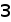
\includegraphics[scale=0.3]{./Figures/Project2/taco/original.png}\\
Interpolation/Extrapolation Without Uncertainty \\
\includegraphics[scale=0.3]{./Figures/Project2/taco/siamese_interp_num.png} \hspace{0.25cm} 
\includegraphics[scale=0.3]{./Figures/Project2/taco/interp_pool_best_reg.png}\\
Interpolation/Extrapolation With Uncertainty \\
\includegraphics[scale=0.3]{./Figures/Project2/taco/interp_nodelta.png} \hspace{0.25cm} 
\includegraphics[scale=0.3]{./Figures/Project2/taco/interp_delta.png}\\
\end{centering} 
\end{frame} 

\begin{frame}
\begin{center} 
\huge \color{blue} \emph{Thank You!}
\end{center} 
\end{frame}


\end{document}

